%\lhead{Modulok es kapcsolatok}

\section{Alacsony szintű modulok} 

A roboton alacsony szintű feladatait amelyek a motor hajtásokhoz kapcsolódó szenzorokat és vezérlő jelek előállítására hivatott a két CmodA7 20T FPGA fejlesztőlap. Négy tengely szögsebességet kell szabályozni, egy FPGA két hajtást valósít meg. A \ref{fig:CmodA7architektura} alapján egy hajtáshoz tartozó I/O-k:

\begin{table}[H]
\center
\begin{tabular}{lll}
\hline Név                            & Darabszám              & Típus  \\ \hline
Inkrementális szenzor           & 2           & Digitális Input \\
Árammérő szenzor                & 1                  & Analóg Input \\
Motor vezérlő                   & 3                  & Digitális Output \\
Végállás kapcsoló                 & 1                  & Digitális Input        
\end{tabular}
\end{table}




\renewcommand{\img}{SajatRobot/SzerkAbrak/cmoda7modulok.jpg}
\renewcommand{\sources}{*}
\renewcommand{\captionn}{CmodA7 FPGA-ban kialakított architektúra amely a szenzorok és motor hajtások jeleinek feldolgozását és előállítását valósítja meg }
\renewcommand{\figlabel}{CmodA7architektura}
\begin{kep}
\begin{figure}[H]
\centering
\ifthenelse{\equal{\svg}{*}}
{
    \includegraphics[width=\aspectratioPic\textwidth,angle=\rotationAnglePic]{\img}
}
{
    \includesvg[width=\aspectratioPic\textwidth,angle=\rotationAnglePic]{\img}
}

 \ifthenelse{\equal{\sources}{*}}
    { \captionof{figure}{ \captionn}}
    { \captionof{figure}{ \mand{\mand{\captionn}{Forrás:}}{}} }
  	

\ifthenelse{\equal{\figlabel}{*}}
    {}
    {\label{fig:\figlabel}}%
    
\renewcommand{\figlabel}{*}



\end{figure}
\end{kep}
\renewcommand{\aspectratioPic}{1}
\renewcommand{\rotationAnglePic}{0}
\renewcommand{\svg}{*}



A \ref{fig:VivadoHl} a Vivado tervezőprogramban FPGA-ban megvalósított processzor architektúra látható, tartalmaz egy szoftcore processzort (microBlaze). Az utasítás és az adatmemória az $microblaze\_0\_local\_memory$-ban található. A memória mérete 24Kbyte 32bit sávszélességgel, amely az FPGA block memóriájából van összerakva. A programkód maga egy külső memóriában van tarolva, QSPI alapú interfésszel kapcsolódik a FPGA hoz, az $ExternalMemorys$ kapcsolja be az AXI busz rendszeren keresztül a processzor memória címtartományába. A külső memória mérete 30 MByte. A processzor működéséhez szükséges a $ClockAndReset$ modul előállítja az órajelet ami 100 MHz, ezen a frekvencián működik az processzor és a memória is. Az $mdm\_1$ modul a rendszerben jeleinek és a programkód megfigyelésére hivatott.

A \ref{fig:VivadoHl} ábrán látható $UartCom$ modul belső szerkezete látható az \ref{fig:UartComVivaldo} ábrán. A modul $uartcommand\_0$ szerepe a kommunikációs protokoll implementálása hardveres szinten, a modul fogadja az UART protokollon  érkező 8 bites csomagokat. A protokoll által meghatározott keretezési byte-okat figyelve (Start,Stop,Skip). Ezek paraméterként megadhatok a microBlaze processzoron keresztül. A processzor induláskor beállítja ezeket a következő értékekre: Start='S', Stop='P', és Skip='\\'. 
Start keret byte érkezésétől kezdve az összes byte négyesével bekerül a 32 bit, 400 byteos, $blk\_mem\_gen\_0$ memóriába jogfolytonosan. Abban az esetben ha az üzenet meghaladja a 200 byte-t akkor a modul úgy tekinti hogy hibás adatok érkeztek és visszatérte a kiinduló állapotba. Abban az esetben ha bináris adatokat küldünk tartalmazhat speciális protokoll keretezésben résztvevő karaktereket így ezeket előtt Skip karakter kell hogy legyen. A skip karakterek nem kerülnek bele a memóriába ezeket a hardver kiveszi és az utána következő karaktert nem értelmezi.

A kommunikáció folyamatát a \ref{fig:FPGAuartRos} ábra is végigkövethetjük.

\begin{figure}[H]		
		%trim = bal also jobb felso
   \fbox{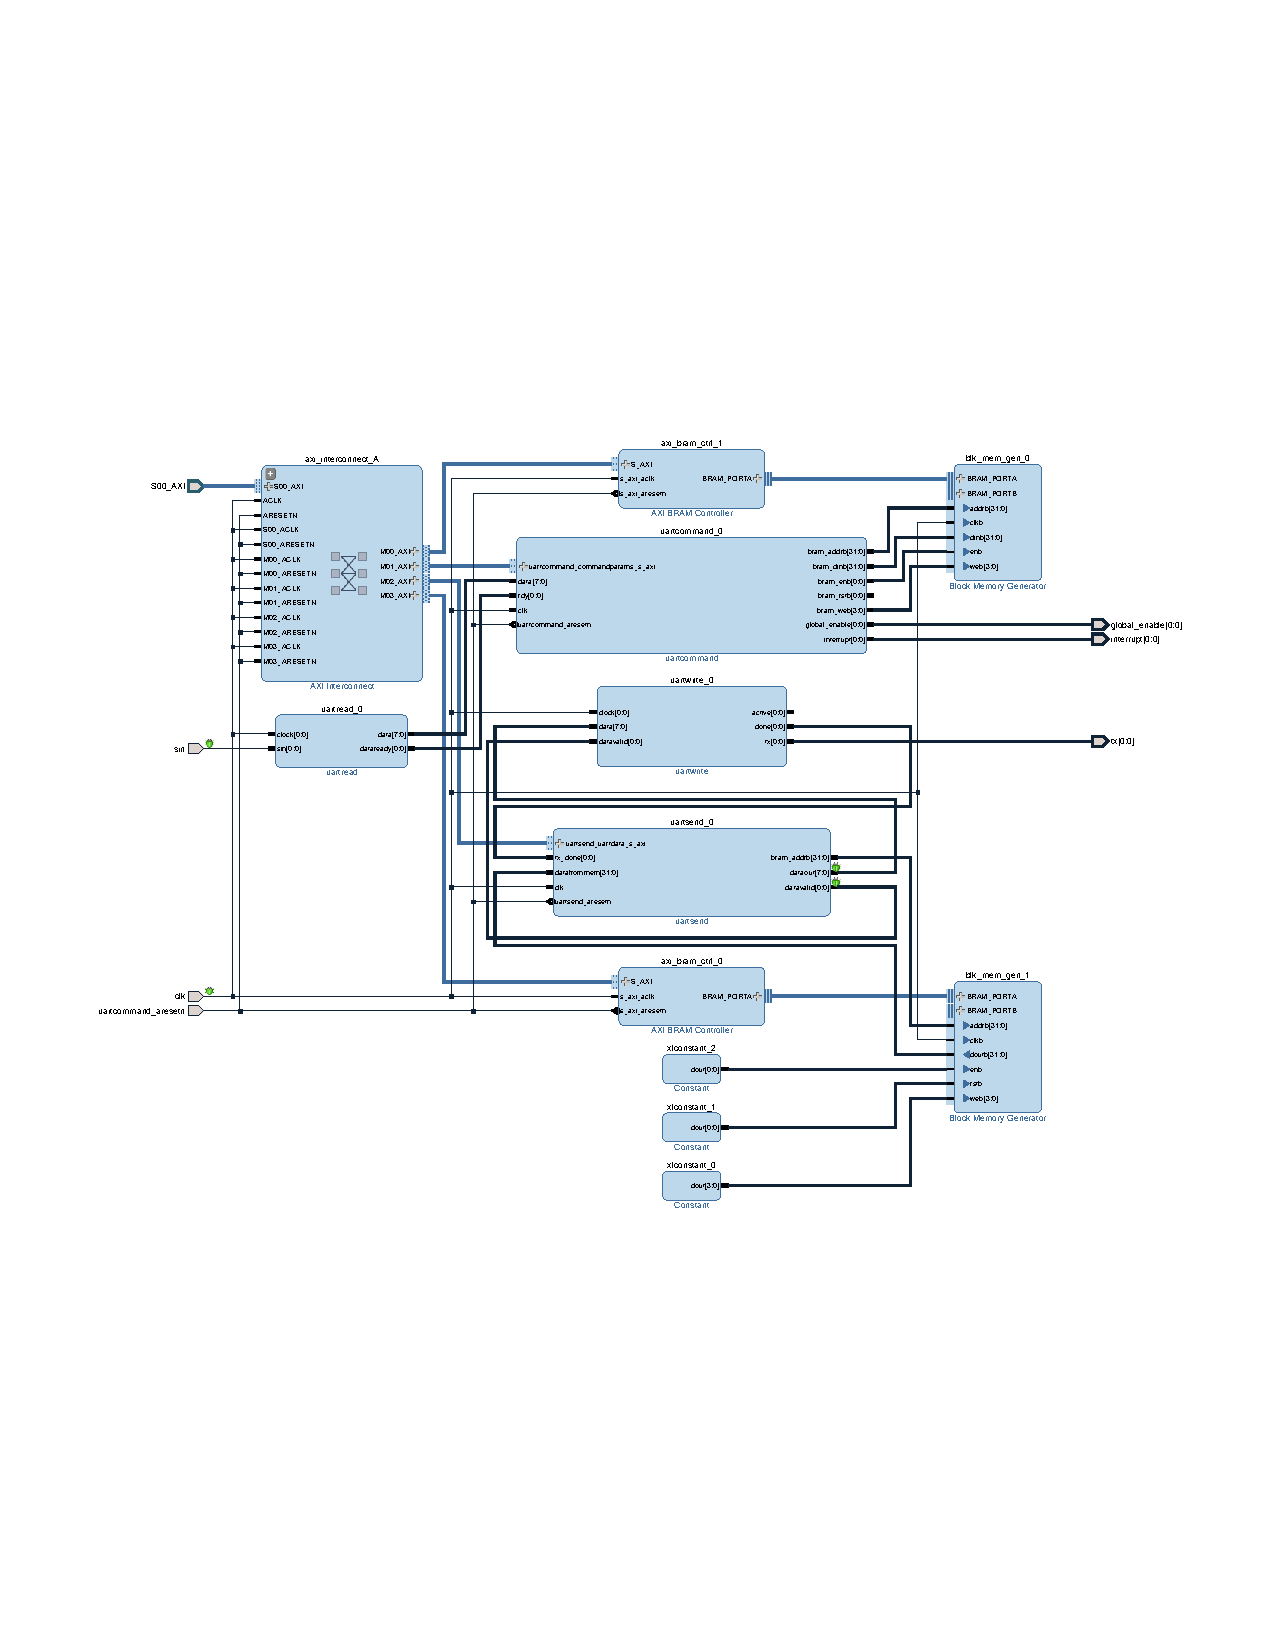
\includegraphics[width=1.1\columnwidth,trim=3cm 7cm 1cm 7cm,clip]{tikz/UartCom.pdf}}
  \caption{FPGA ban megvalósított kommunikációs modul a 	     \ref{fig:FPGAcomuSection} leírt protokoll alapján.}
  \label{fig:UartComVivaldo}
\end{figure}


\renewcommand{\img}{SajatRobot/FPGAmodulok/UartUML.jpg}
\renewcommand{\sources}{*}
\renewcommand{\captionn}{FPGA hardver/MicroBlaze processzor és ROS node közti kommunikáció megvalósítása UART protokoll alapján }
\renewcommand{\figlabel}{FPGAuartRos}
\begin{kep}
\begin{figure}[H]
\centering
\ifthenelse{\equal{\svg}{*}}
{
    \includegraphics[width=\aspectratioPic\textwidth,angle=\rotationAnglePic]{\img}
}
{
    \includesvg[width=\aspectratioPic\textwidth,angle=\rotationAnglePic]{\img}
}

 \ifthenelse{\equal{\sources}{*}}
    { \captionof{figure}{ \captionn}}
    { \captionof{figure}{ \mand{\mand{\captionn}{Forrás:}}{}} }
  	

\ifthenelse{\equal{\figlabel}{*}}
    {}
    {\label{fig:\figlabel}}%
    
\renewcommand{\figlabel}{*}



\end{figure}
\end{kep}
\renewcommand{\aspectratioPic}{1}
\renewcommand{\rotationAnglePic}{0}
\renewcommand{\svg}{*}


\begin{figure}[H]
  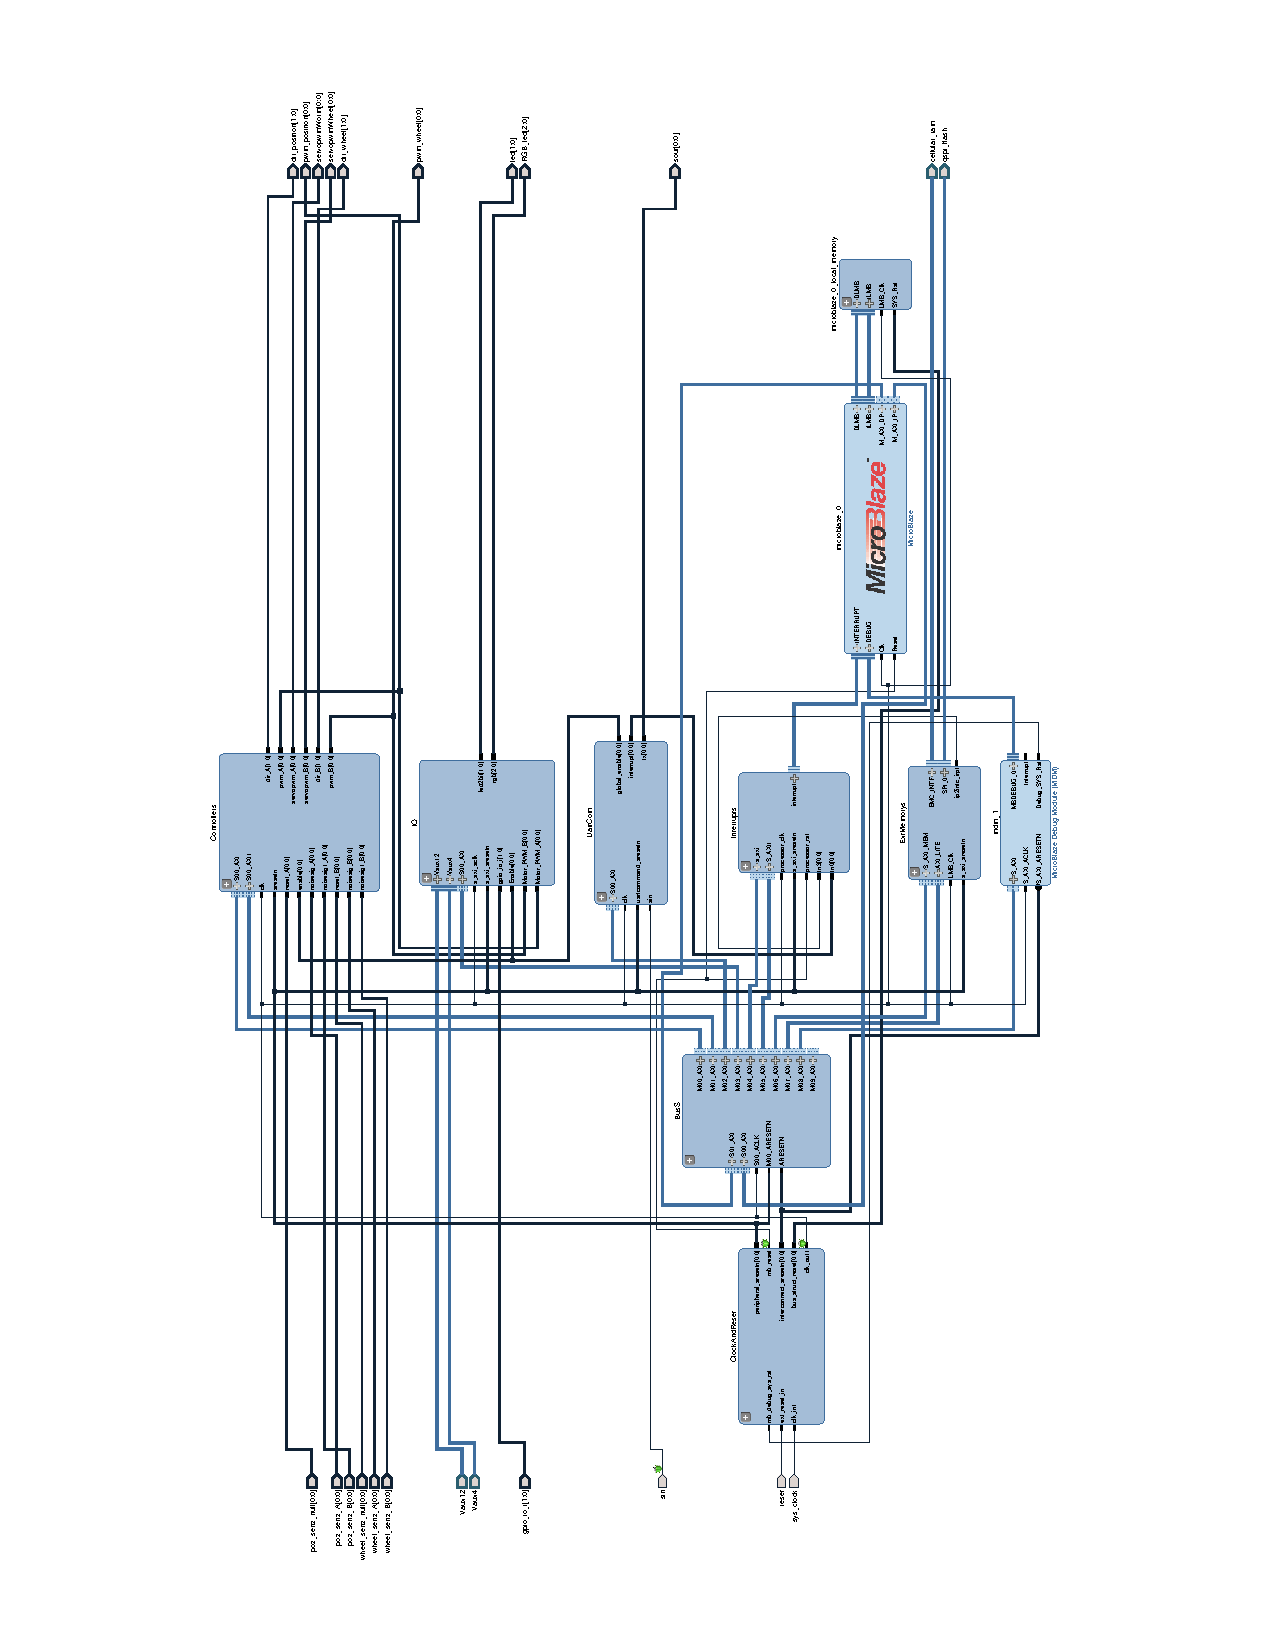
\includegraphics[width=1.2\columnwidth]{tikz/VivadoHL.pdf}
  \caption{FPGA ban megvalósított szoftprocesszor rendszer, legfelső négyzete.}
  \label{fig:VivadoHl}
\end{figure}

A keret véget jelző byte érkezésekor a modul generál egy megszakítást a microBlaze processzornak az $interupt[0:0]$ kivezetésen keresztül.
A megszakítás kiszolgálásakor a processzor kiolvassa az $uartcommand_0$ modulból az új üzenet kezdőcímét. A processzor az adatokat az $axi\_bram\_ctrl\_1$ modulon keresztül kepés kiolvasni, az új üzenetre kezdőcímére, mutató pointer értékét megkapjuk, ha az $uartcommand_0$ modul processzor memóriájába illesztésétt kezdőcímét és a modul által jelzet kezdőcímet összeadjuk.
Abban az esetben, ha az adatok feldolgozása előtt új csomag érkezik a hardver kommunikációs modulhoz, elkezdődik annak beírása a memóriába, az előző adatok felülírás nélkül.

A $uartcommand_0$ modul kimenete $global\_enable[0:0]$ engedélyező jel, abban az esetben ha nem kap a hardver $SREP$ üzenetet legalább 300ms periódussal, akkor az engedélyező jelet alacsonyra állítja vagy ha $SRDP$ üzenet érkezett.

Az $uartsend\_0$ modul hasonlokeppen müködik csak az adatok küldésére hivatott. A microBlaze proceszor az $axi\_bram\_ctrl\_0$ modulon keresztül beleirodnak a $blk\_mem\_gen\_1$ \cite{DualPortRam} 32bites és 400byte méretű memóriába.
Az írás végével a processzor beállítja a küldés jelet, amely egy paramétere a hardvernek. A modul elkezdi kiküldeni az adatokat. Abban az esetben ha a csomag tartalmaz speciális protokollt leíró byte-t akkor a modul automatikusan elküldi előtte a Skip karaktert.

Az $uartread\_0$ az UART protokoll implementálja FPGA hardverebe, a $sin$ az RX bemenet, a $data[7:0]$ a 8 bites szeles adatvezeték ami tartalmazza az utolsó beérkeztt byte-t. A $dataready[0:0]$ felfutó él jelzi az új adat érkezését. Az $uartwrite\_0$ modul a $data[7:0]$ 8bites sinen érkező adatot küldi ki UART protokoll alapján a $tx[0:0]$ kimenetere abban az esetben ha a $datavalid[0:0]$ bemenetén egy felfutó él érkezik.

Az \ref{fig:ControllersVivado} látható $A$ és $B$ modul feladatuk egy-egy DC motor szabályzását/vezérlését lássák el. Mindkét modulban ugyan azon alegységek találhatok meg az $A$ modul az robot első, míg a $B$ modul a robot hátsó kerekét szabályozza.

A \ref{fig:ControllerMag} ábrán látható az $A$ és $B$ modulok belső szerkezete. A $pwm\_hardver\_B$ PWM jelet állít elő, a $pwm[0:0]$ kimenetre, és egy irányjelet $dir[0:0]$, a bemeneti 16bites előjeles számból áll. A PWM kitöltési tényezője -32000 tol 32000-ig terjed ki (15bit), az előjel meghatározza az irányt míg az abszolút érteke a pwm kitöltési értéket. A $enable[0:0]$ jel engedélyezi a kimenetet, ha érteke alacsony akkor a pwm kimenet is alacsony.


\begin{figure}[H]
  		%trim = bal also jobb felso
   \fbox{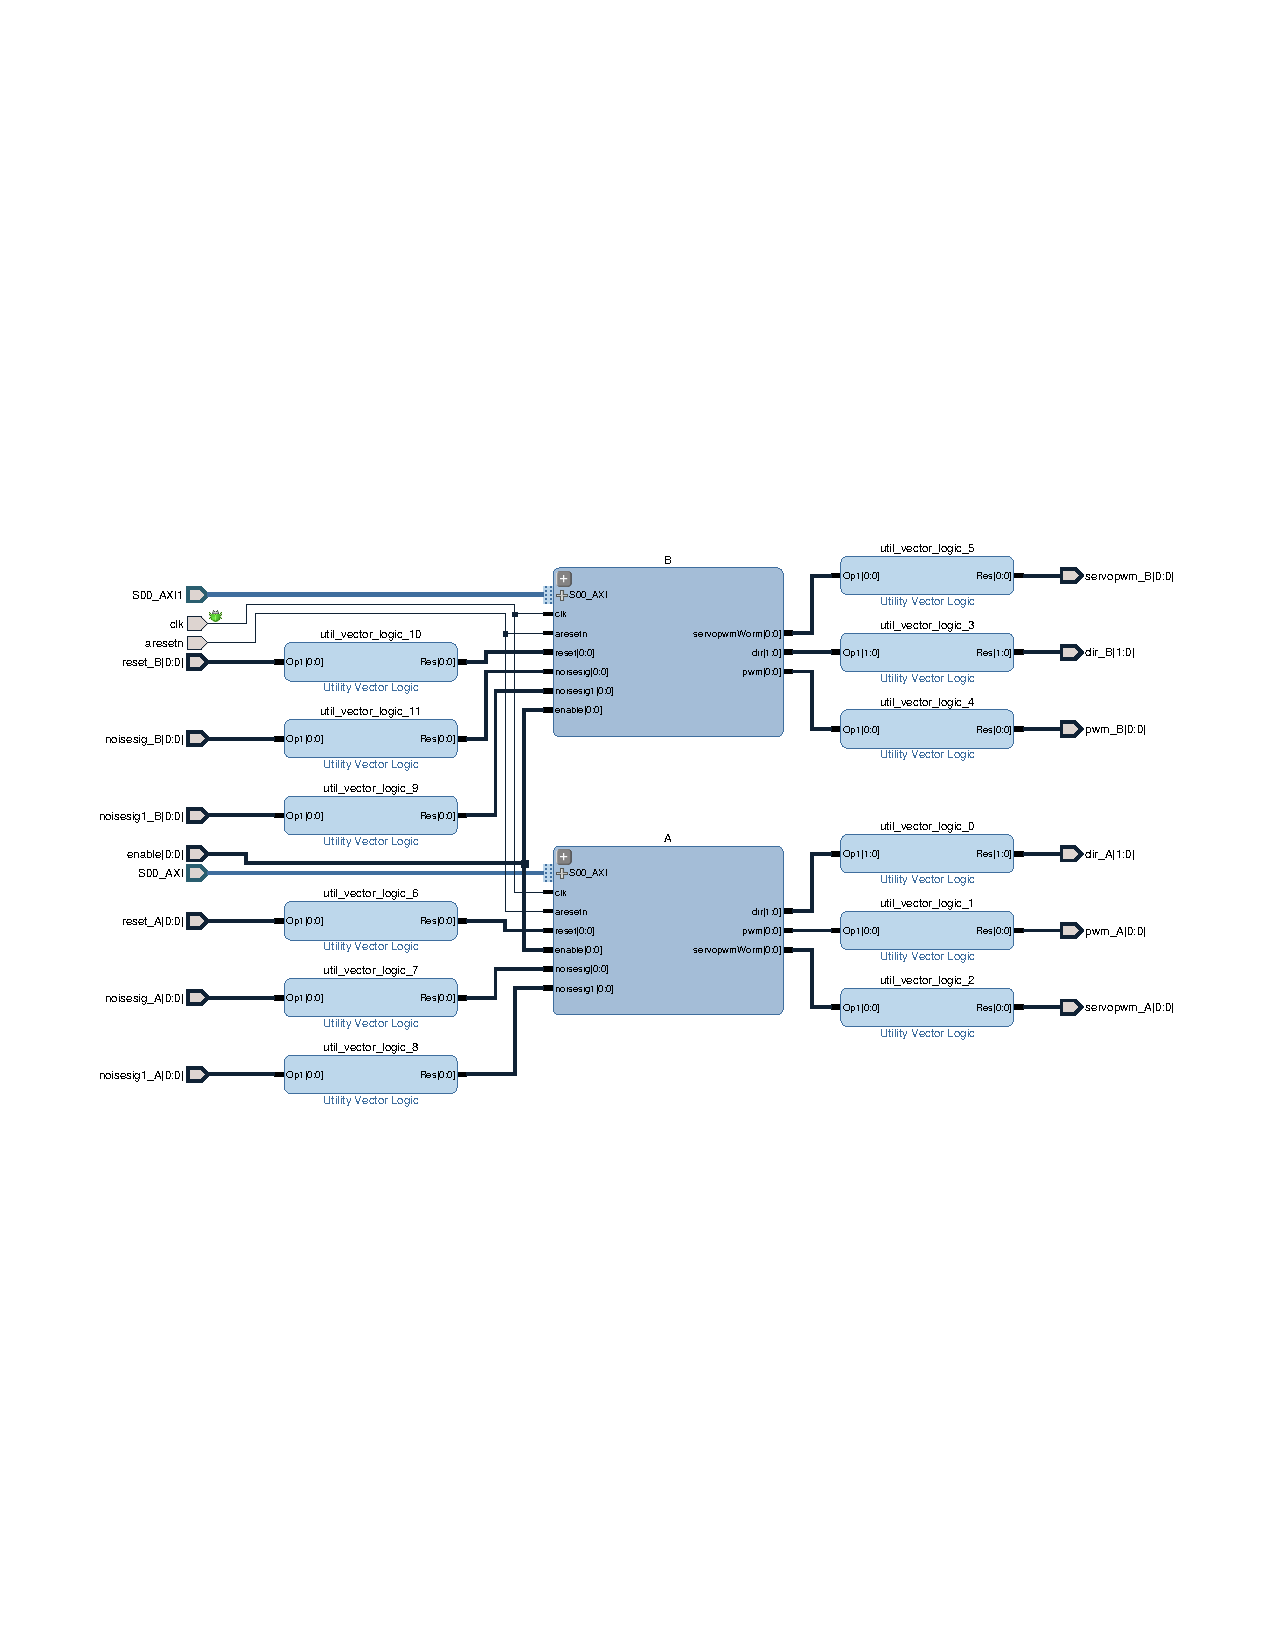
\includegraphics[width=1.1\columnwidth,trim=2cm 9cm 1cm 9cm,clip]{tikz/Controllers.pdf}}
  \caption{FPGA-ban megvalósított szabályzok A és B}
  \label{fig:ControllersVivado}
\end{figure}

Az $InkrementalisSensor\_B$ axi sínen keresztül kapcsolódik a processzorhoz, feladata az inkrementális szenzortól érkező $A$ és $B$ jeleknek a feldolgozása. A modul két jelet küld ki: $dir[0:0]$ amely a tengely forgás irányát jelzi, $imp[0:0]$ egy órajelperidusig tartó felfutójelet küld ki az inkrementális szenzor minden egyes elmozdulására.
\begin{figure}[H]
    		%trim = bal also jobb felso
   \fbox{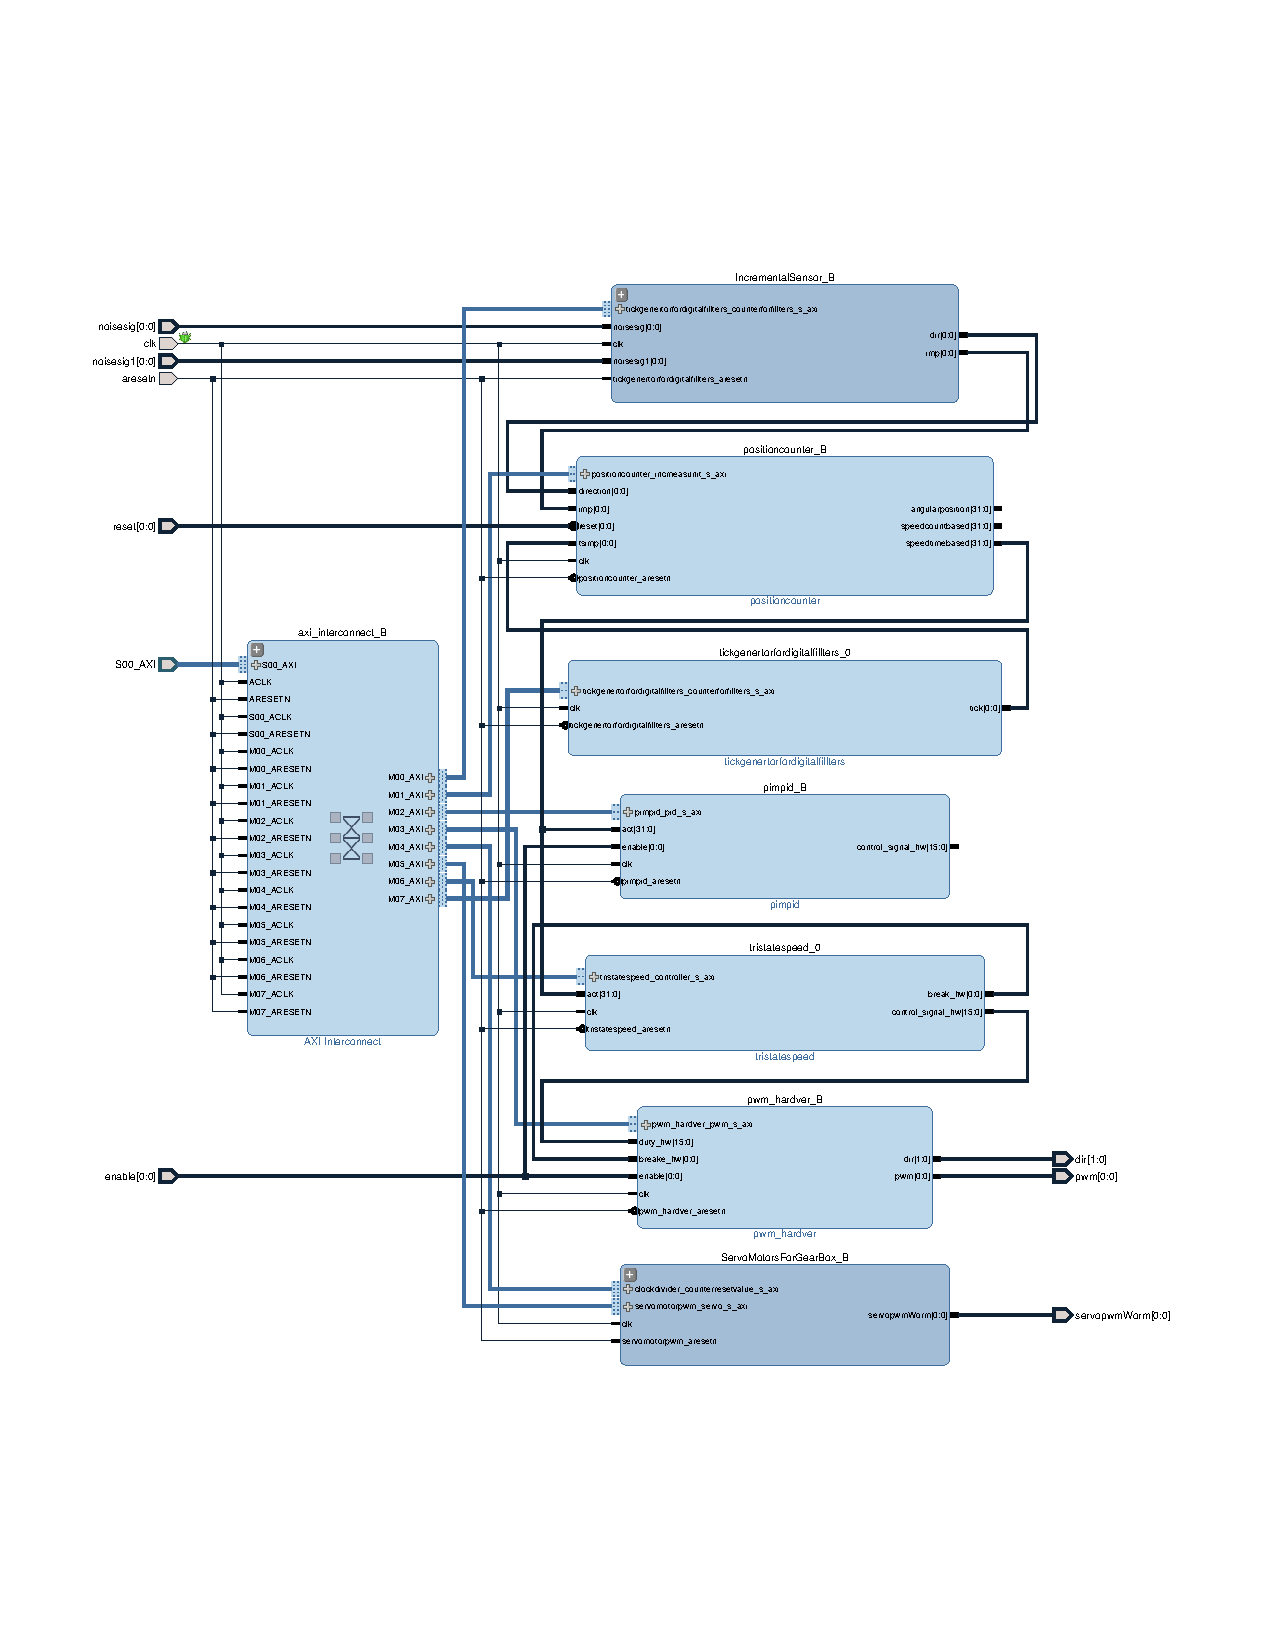
\includegraphics[width=1.1\columnwidth,trim=1cm 4cm 1.8cm 4cm,clip]{tikz/B.pdf}}
  \caption{FPGA controller modul}
  \label{fig:ControllerMag}
\end{figure}

A $positioncounter\_B$ modul meri a szögsebességet és a szögpozíciót idő és impulzus számolási módszert használva. A processzor a saját mintavételezési frekvenciájával olvassa ki a modulból a mert értékeket és átalakítja kivant mértékegységbe.

Az \ref{fig:ControllerMag} ábrán látható többi modul jelen pillanatban továbbfejlesztési lehetőségként jelenik meg. A $pimpid\_B$ modul FPGA alapú PID szabályzó modul, $ServoMotorGearBox\_B$ a DC motrokon levő fogaskerék kapcsolási lehetőséget hivatott majd állítani egy szervomotor segítségével.

A szabályzok referencia értékeit a $RefValues$ funkcionalitás biztosítja, a megfelelő üzenetek érkezésekor a memóriába beállítódnak a kívánt referencia értékek, és majd a szoftveres szabályzok kiolvassák. A hardveres szabályzóknak pedig a beérkezés pillanatban leküldődik.

A $Monitors/Controllers$ funkcionalitas egy parameterbol allithato periodusu idozito amely megszakitasokat general a proceszornak. A proceszor ezekre a megszakitasokra szamolja ki a beavatkozi jelek uj ertekeit, valamint a elkuldi a mert,es a kapott referencia erteketk UART on keresztul.



\subsection{Microblaze szoftvere}

A rendszer tervezésénél a fő koncepció az volt hogy a rendszer architekturája dinamikus legyen a fejleszthetőséget tekintve, így a \ref{fig:CmodA7architektura} levő arhitekurát kaptuk.

A microblaze processzor feladatai hardveres modulok kezdeti állapotainak a beállítása, szoftveresen futó szabályzók működtetése, a beérkezett üzenetek feldolgozása. A processzoron futó szoftvert az \ref{fig:MicroblazeSoft} UML diagram szemlélteti.
A paraméterek írása és olvasása funkcionalitásban, az új beérkezet paraméter értekének a beállítási mente a következő: az üzenet beleíródik a memóriába, megszakítás generálódik a processzor irányában, a processzor feldolgozza az új üzenetet, észleli hogy paraméter értekének a beállítása típusú üzenet érkezett, meghívódik a kiszolgáló függvény. A továbbiakban az összes paraméter újraszámolódik, és újraküldődik a hardveres modulok irányába. Abban az esetben ha minden sikeresen beállítódott a processzor pozitív visszajelzést(ACK) üzenetet küld és visszaküldi a beállított paraméter értékét, acélból hogy a küldő is megbizonyosodjon a paraméter helyes beállításáról.


\renewcommand{\img}{SajatRobot/FPGAmodulok/uBlazeAndFpgaUML.jpg}
\renewcommand{\sources}{*}
\renewcommand{\captionn}{MicroBlaze processzoron futó szoftver diagramja}
\renewcommand{\figlabel}{MicroblazeSoft}
\begin{kep}
\begin{figure}[H]
\centering
\ifthenelse{\equal{\svg}{*}}
{
    \includegraphics[width=\aspectratioPic\textwidth,angle=\rotationAnglePic]{\img}
}
{
    \includesvg[width=\aspectratioPic\textwidth,angle=\rotationAnglePic]{\img}
}

 \ifthenelse{\equal{\sources}{*}}
    { \captionof{figure}{ \captionn}}
    { \captionof{figure}{ \mand{\mand{\captionn}{Forrás:}}{}} }
  	

\ifthenelse{\equal{\figlabel}{*}}
    {}
    {\label{fig:\figlabel}}%
    
\renewcommand{\figlabel}{*}



\end{figure}
\end{kep}
\renewcommand{\aspectratioPic}{1}
\renewcommand{\rotationAnglePic}{0}
\renewcommand{\svg}{*}





\subsection{FPGA és UART alapú kommunikációs protokoll}
\label{FPGAcomuSection}
Megvalósítva a kommunikációt a kiszolgáló ROS-node, amely UART protokollra épített saját üzenetekből áll. \ref{fig:FPGAComCsomagAlt}.

\renewcommand{\img}{SajatRobot/FPGAmodulok/ProtokolDiagram.jpg}
\renewcommand{\sources}{*}
\renewcommand{\captionn}{FPGA komunikacios protokol altalanos csomag szerkezet}
\renewcommand{\figlabel}{FPGAComCsomagAlt}
\begin{kep}
\begin{figure}[H]
\centering
\ifthenelse{\equal{\svg}{*}}
{
    \includegraphics[width=\aspectratioPic\textwidth,angle=\rotationAnglePic]{\img}
}
{
    \includesvg[width=\aspectratioPic\textwidth,angle=\rotationAnglePic]{\img}
}

 \ifthenelse{\equal{\sources}{*}}
    { \captionof{figure}{ \captionn}}
    { \captionof{figure}{ \mand{\mand{\captionn}{Forrás:}}{}} }
  	

\ifthenelse{\equal{\figlabel}{*}}
    {}
    {\label{fig:\figlabel}}%
    
\renewcommand{\figlabel}{*}



\end{figure}
\end{kep}
\renewcommand{\aspectratioPic}{1}
\renewcommand{\rotationAnglePic}{0}
\renewcommand{\svg}{*}



A protokoll keretek közé foglalt adatok rendiségre épül. Speciális karakterek \footnote{speciális karakterek amelyek jelzik az értelmező szamara hogy olyan karakter következik amelyet a protokoll értelmezésében nem kell végrehajtani.} jelzik az üzenet kezdetet és véget jelen esetben az $S$ csomag kezdetét, míg a $P$ a csomag véget jelentik.
Az csomag tartalmazhat bináris formátumú adatot is ezeket minden esetben a \{ és \} speciális karakterek közé kel kerülniük, mert a köztük levő adat nem fog értelmezésre kerülni a feldolgozó által. Bináris reszt  pl:. struktúra típusú adatra használhatjuk. Mindig a \{ utáni első karakter megadja a bináris adat hosszát így tudja az értelmező hogy hol kell várnia a lezáró karaktert. A bináris szekció hossza nem lehet nagyobb mint 254 byte, de amennyiben szükséges kiterjeszthető.

Minden üzenet tartalmaz egy egyedi azonosítót ami meghatározza az üzenet típusát ez alapján tudja eldönteni majd a fogadott fél hogy melyik kiszolgáló rutint kell felhívnia. Ezt követi egy üzenet számláló 5 char hószú mező amely string formában tartalmaz egy egész számot, amely minden kiküldött üzenet után növelni kell. Az üzenetszámlaló alól kivételt kepéznek a direkt hardveres üzenetek pl.: $SREP$ és a $SRDP$.
A hasznos adat további felépítését meghatározható annak függvényében hogy mit szeretnénk. Jelen esetben a üzenet típus orientált parancsokat szerkesztünk amelyekkel a referencia értékeket, paramétereket állítjuk be, valamint bináris szekciót is tartalmazó struktúrát küld az FPGA modul PC-nek amely a szabályzást és historizálást szolgálja.

\subsection{Paraméterek FPGA modul}

A paraméterek segítségével tudjuk beállítani a mintavételezési periódusokat, az inkrementális szenzorok felbontását, a szabályozok beállítását is ezáltal oldhatjuk meg.
Konfigurációs paraméterek:
Az alábbi táblázatban leírjuk a ROS-ban használt paramétereket. A paraméterek nevének végen levő $X$ jelölje $A$ vagy $B$, attól függően hogy melyik DC motorhajtáshoz tartozik. Az \ref{fig:ControllersVivado} ábrán látható modulokat tudjuk konfigurálni.
% Please add the following required packages to your document preamble:
% \usepackage{multirow}
% \usepackage[normalem]{ulem}
% \useunder{\uline}{\ul}{}

\begin{table}[H]
\begin{tabular}{lllllp{6cm}}
\hline \multirow{2}{*}{Id} & \multirow{2}{*}{\begin{tabular}[c]{@{}l@{}}Név \\ (X lehet A vagy B)\end{tabular}} & \multicolumn{2}{l}{Értékek} & \multirow{2}{*}{Típus} & \multirow{2}{*}{Leírás}                                                                                                                      \\
                    &                                                                                    & Min         & Max           &                        &                                                                                                                                              \\ \hline
1                   & TsTimerPeriod                                                                      & 1           & 1000          & int16                  &  Mintavételezési periódus {[}ms{]} ban.                                                                                                      \\
2                   & GetDataPeriodical                                                                  & 0           & 1             & int16                  &  Kapcsoló ha 0 akkor nem küld az FPGA mért értékeket, különben a TsTimerPeriod periódusú mintavétellel küld.                                  \\
3                   & TorqueCoefX                                                                        &             &               & float16                &  Motor arám és nyomaték közti együttható.                                                                                                      \\
4                   & ActiveControllerX                                                                  & 0           & 65535         & int16                  &  Válaszható szabályzó típusok hajtásonként 0=Szoftvare PID szögsebesség, 1=Hardver PID szögsebesség, 2=Szoftver PID arám, 3=Hardver PID arám  \\
5                   & MaxControlSiggnalX                                                                 & 0           & 32760         & sint16                 &  A beavatkozó PWM jel maximális kitöltési tényezője, lineárisan 0-\textgreater{}0\% -tol 32760-\textgreater{}100\% -ig.                       \\
6                   & IncSenzResX                                                                        & 0           & 65535         & int16                  &  Inkrementális szenzor által generált impulzusok száma egy teljes kerékfordulatra. FPGA oldalon ez a szám 10-el szorzandóik.                     \\
7                   & IncSenzCountDirectionX                                                             & -1          & 1             & sint16                 &  Inkrementális szenzor jeleit feldolgozó modul számolási iránya állítható be.                                          \\
8                   & Kp\_Whell\_PidX                                                                    & 0           &               & float16                &  szögsebesség szabályzó, PID erősítési paramétere.                                                                                             \\
9                   & Ti\_Whell\_PidX                                                                    &             &               & float16                &  szögsebesség szabályzó, PID integrálási idő.                                                                                                  \\
10                  & Td\_Whell\_PidX                                                                    &             &               & float16                &  szögsebesség szabályzó, PID deriválási idő.                                                                                                   
\end{tabular}
\end{table}






\subsection{Kommunikáció sebessége}

Az uart sebessége 1MBd \footnote{megabaud} ami megfelel 131072 byte/s adatforgalomnak. A valosagban a komunikáció hibátlanul müködik 1 ms periodussal, küldött 100byte méretü üzeneteket. Összehasonlítva $AXI\_UART\_Lite$ \cite{AXIuartLite} modullal elért eredmények, 50 ms periódust tudtunk csak elérni, mert a protokoll értelmezését a szoftver végezte és nem a hardver. A FIFO használata ellenére sem sikerült kisebb mintavételezési periódust elérni, hogy nem minden karakter után generált processzor megszakítást csak minden 16-dik karakter után.

\begin{equation}
    frekvencia = \frac{131072}{SizeOfPachage}=\frac{131072[byte/s]}{100[byte]}=1310,072 [Hz]
\end{equation}

\subsection{Biztonsági megoldások}

Abban az esetben ha kiküldtük az előírt értékeket a modulnak és ezután a kommunikáció megszakadt a modullal akkor a szabályzok próbáljak tartani az előírt érteket annak ellenére is hogy az mar lehet hogy nem aktuális. Erre a célra beépitésre került egy üzenet és egy logika (HeartBeat), a periodikusan érkező üzenet, amely csak a kommunikációs modulhoz érkezik meg, és jelzi hogy a ROS jól működik, és fordítva is küldődik periodikus üzenet amely jelzi az FPGA normális működést. Abban az esetben ha a  megszakad leállítja a motorokat és a szabályzókat,  \ref{fig:FPGAuartRos} alapján az Enable(EN) jelet használva.

\begin{table}[H]
\center
\begin{tabular}{lll}
\hline Irány   & Üzenet & Periódus    \\ \hline
FPGA->ROS &  SEP        & 300 ms kötelező         \\
ROS->FPGA &  mintavételezett értékek küldése & dinamikusan módosítható                   
\end{tabular}
\end{table}
